% Chapter 5

\chapter{The critical temperature} % Main chapter title

\label{Chapter6} % For referencing the chapter elsewhere, use \ref{Chapter3} 

\lhead{Chapter 6. \emph{The critical temperature}} % This is for the header on each page - perhaps a shortened title

%----------------------------------------------------------------------------------------
In this chapter we will first derive a linearized gap equation, see section \ref{sec.linearizedgapequation}. This will give us a more efficient way of calculating the critical temperature $T_C$ for the transition between the superconducting and normal phase. In section \ref{sec.criticaltemperature.numerical} we will then solve the equation numerically and investigate the dependency of $T_C$ on gas parameters $(n_Ba_{BF}^3)^{1/3}$ and $(n_Ba_B^3)^{1/3}$. 

\section{The linearized gap equation} \label{sec.linearizedgapequation}
In the analysis of chapter \ref{Chapter5} the estimation of the critical temperature $T_C$ is quite tedious. We have to wait for an increasing number of iterations near $T_C$ to get a good estimate and calculating the critical temperature as a function of the parameters of the problem is out of the question. In this section we will describe a much more efficient way of estimating the critical temperature through \textit{the linearized gap equation}. This in turn will be performed in section \ref{sec.criticaltemperature.numerical}, where the goal is to calculate the dependency of $T_C$ on the gas parameters.

The gap equation in its full integral form is (see equation \eqref{eq.GapequationIntegral}):
\begin{equation}
\Delta_k = - \int \frac{dk'}{2\pi} W^\text{ind}_{FF}(k,k')\frac{\tanh\left(\frac{\beta E_{F,k}}{2}\right)}{2E_{F,k'}}\Delta_{k'}. \nonumber
\end{equation} 
As we saw in chapter \ref{Chapter5} the gap goes to zero at the critical temperature $T_C$: $\Delta_k(T_C) = 0$. The energy $E_{F,k} = \sqrt{\epsilon_k^2 + |\Delta_k|^2}$ is quadratic in the gap. It follows that by only retaining the gap to first order, we obtain a linear equation near $T_C$:
\begin{equation}
\Delta_k = - \int \frac{dk'}{2\pi} W^\text{ind}_{FF}(k,k')\frac{\tanh\left(\frac{\beta \varepsilon_k}{2}\right)}{2\varepsilon_k} \Delta_{k'}.
\label{eq.GapequationIntegralLinear}
\end{equation} 
Here we have also used, that $\frac{\tanh\left(\frac{\beta \varepsilon_k}{2}\right)}{2\varepsilon_k}$ is even in $\varepsilon_k$, so that the absolute value stemming from the square root can be omitted. This defines a linear equation with eigenvalue $1$: $\Delta_k = L(\Delta_k)$. $L$ is then a linear transformation defined by the integral above. Hence, the program for the evaluation of $T_C$ is now clear. Since $L$ is an integral operator, the eigenvalues of $L$ will form a continuum. Thus, to find $T_C$ we must find the temperature at which the largest eigenvalue becomes unity. 


\section{Calculating the critical temperature} \label{sec.criticaltemperature.numerical}
In this section we will describe how in practice to perform the calculation outlined in the above. 

To do the calculation in practice we need to but the linear equation on matrix form. From equation \eqref{eq.GapequationIntegralLinear} it is clear, that we have the matrix equation:
\begin{equation}
\Delta_k = L \Delta_k, \hspace{0.5cm} L(k,k') = -\frac{dk'}{2\pi} W^\text{ind}_{FF}(k,k')\frac{\tanh(\beta \varepsilon_{k'}/2)}{2\varepsilon_{k'}}. 
\label{eq.Gapmatrixequation}
\end{equation}
Explicitly we define a cutoff $k_{up}$ and spacing $dk'$. We then need to make $k_{up}$ large enough and $dk'$ small enough for the eigenvalues to have converged. From the form of $L(k,k')$ it is also clear, that $L$ is not a symmetric matrix; each row of $L$ has all the possible values of $\varepsilon_{k'}$, but each column only has a single value belonging to the entire column. The evaluation is performed in MatLab in the following fashion. For a fixed set of parameters we start out with an initial guess $T$ for $T_C$, that we know is too high. We then iteratively decrease $T$ by a small amount $dT$ and calculate the largest eigenvalue for each iteration. When the largest eigenvalue becomes larger than 1, we halt the iteration and set the critical temperature to the current value of $T$. The numerical analysis is a balancing act. We have to choose a resolution fine enough, defined by $dk'$ and $k_{up}$, for the eigenvalues to have converged to the eigenvalue for the integral operator, and still keep the matrix $L$ small enough for the analysis to be feasible. In this context it is crucial that we have a closed form expression for $W^\text{ind}_{FF}(k,k')$ in the $l_t \to 0$ limit. 

In figure \ref{fig.TCrB} we see the dependency of $T_C$ on the Bose gas parameter $(n_Ba_B^3)^{1/3}$. We observe a simple monotonic decrease with increasing gas parameter. Physically this can be understood in the following way. When $(n_Ba_B^3)^{1/3}$ is increased for $\frac{n_F}{n_B^{1/3}}$ fixed, the BEC coherence length $k_F\xi = \frac{\pi}{\sqrt{8 n_B/n_F^3 k_Fa_B}}$ decreases. The coherence length is the range of the interaction in real space: $\tilde{V_{FF}^{\text{ind}}} \propto \frac{ \text{e}^{ -\sqrt{2}|x|/\xi } } {|x|}$. Therefore the interaction range is decreased, when we increase $(n_Ba_B^3)^{1/3}$, and so it is physically reasonable, that the critical temperature goes down with increasing $(n_Ba_B^3)^{1/3}$.

\begin{figure} 
\begin{center}  
% GNUPLOT: LaTeX picture with Postscript
\begingroup
  \makeatletter
  \providecommand\color[2][]{%
    \GenericError{(gnuplot) \space\space\space\@spaces}{%
      Package color not loaded in conjunction with
      terminal option `colourtext'%
    }{See the gnuplot documentation for explanation.%
    }{Either use 'blacktext' in gnuplot or load the package
      color.sty in LaTeX.}%
    \renewcommand\color[2][]{}%
  }%
  \providecommand\includegraphics[2][]{%
    \GenericError{(gnuplot) \space\space\space\@spaces}{%
      Package graphicx or graphics not loaded%
    }{See the gnuplot documentation for explanation.%
    }{The gnuplot epslatex terminal needs graphicx.sty or graphics.sty.}%
    \renewcommand\includegraphics[2][]{}%
  }%
  \providecommand\rotatebox[2]{#2}%
  \@ifundefined{ifGPcolor}{%
    \newif\ifGPcolor
    \GPcolorfalse
  }{}%
  \@ifundefined{ifGPblacktext}{%
    \newif\ifGPblacktext
    \GPblacktexttrue
  }{}%
  % define a \g@addto@macro without @ in the name:
  \let\gplgaddtomacro\g@addto@macro
  % define empty templates for all commands taking text:
  \gdef\gplbacktext{}%
  \gdef\gplfronttext{}%
  \makeatother
  \ifGPblacktext
    % no textcolor at all
    \def\colorrgb#1{}%
    \def\colorgray#1{}%
  \else
    % gray or color?
    \ifGPcolor
      \def\colorrgb#1{\color[rgb]{#1}}%
      \def\colorgray#1{\color[gray]{#1}}%
      \expandafter\def\csname LTw\endcsname{\color{white}}%
      \expandafter\def\csname LTb\endcsname{\color{black}}%
      \expandafter\def\csname LTa\endcsname{\color{black}}%
      \expandafter\def\csname LT0\endcsname{\color[rgb]{1,0,0}}%
      \expandafter\def\csname LT1\endcsname{\color[rgb]{0,1,0}}%
      \expandafter\def\csname LT2\endcsname{\color[rgb]{0,0,1}}%
      \expandafter\def\csname LT3\endcsname{\color[rgb]{1,0,1}}%
      \expandafter\def\csname LT4\endcsname{\color[rgb]{0,1,1}}%
      \expandafter\def\csname LT5\endcsname{\color[rgb]{1,1,0}}%
      \expandafter\def\csname LT6\endcsname{\color[rgb]{0,0,0}}%
      \expandafter\def\csname LT7\endcsname{\color[rgb]{1,0.3,0}}%
      \expandafter\def\csname LT8\endcsname{\color[rgb]{0.5,0.5,0.5}}%
    \else
      % gray
      \def\colorrgb#1{\color{black}}%
      \def\colorgray#1{\color[gray]{#1}}%
      \expandafter\def\csname LTw\endcsname{\color{white}}%
      \expandafter\def\csname LTb\endcsname{\color{black}}%
      \expandafter\def\csname LTa\endcsname{\color{black}}%
      \expandafter\def\csname LT0\endcsname{\color{black}}%
      \expandafter\def\csname LT1\endcsname{\color{black}}%
      \expandafter\def\csname LT2\endcsname{\color{black}}%
      \expandafter\def\csname LT3\endcsname{\color{black}}%
      \expandafter\def\csname LT4\endcsname{\color{black}}%
      \expandafter\def\csname LT5\endcsname{\color{black}}%
      \expandafter\def\csname LT6\endcsname{\color{black}}%
      \expandafter\def\csname LT7\endcsname{\color{black}}%
      \expandafter\def\csname LT8\endcsname{\color{black}}%
    \fi
  \fi
    \setlength{\unitlength}{0.0500bp}%
    \ifx\gptboxheight\undefined%
      \newlength{\gptboxheight}%
      \newlength{\gptboxwidth}%
      \newsavebox{\gptboxtext}%
    \fi%
    \setlength{\fboxrule}{0.5pt}%
    \setlength{\fboxsep}{1pt}%
\begin{picture}(7200.00,5040.00)%
    \gplgaddtomacro\gplbacktext{%
      \csname LTb\endcsname%
      \put(946,767){\makebox(0,0)[r]{\strut{}$0$}}%
      \csname LTb\endcsname%
      \put(946,1609){\makebox(0,0)[r]{\strut{}$0.05$}}%
      \csname LTb\endcsname%
      \put(946,2451){\makebox(0,0)[r]{\strut{}$0.1$}}%
      \csname LTb\endcsname%
      \put(946,3292){\makebox(0,0)[r]{\strut{}$0.15$}}%
      \csname LTb\endcsname%
      \put(946,4134){\makebox(0,0)[r]{\strut{}$0.2$}}%
      \csname LTb\endcsname%
      \put(946,4976){\makebox(0,0)[r]{\strut{}$0.25$}}%
      \csname LTb\endcsname%
      \put(1141,484){\makebox(0,0){\strut{}$0.005$}}%
      \csname LTb\endcsname%
      \put(2261,484){\makebox(0,0){\strut{}$0.01$}}%
      \csname LTb\endcsname%
      \put(3381,484){\makebox(0,0){\strut{}$0.015$}}%
      \csname LTb\endcsname%
      \put(4500,484){\makebox(0,0){\strut{}$0.02$}}%
      \csname LTb\endcsname%
      \put(5620,484){\makebox(0,0){\strut{}$0.025$}}%
      \csname LTb\endcsname%
      \put(6740,484){\makebox(0,0){\strut{}$0.03$}}%
    }%
    \gplgaddtomacro\gplfronttext{%
      \csname LTb\endcsname%
      \put(176,2871){\rotatebox{-270}{\makebox(0,0){\strut{}$(n_Ba_B^3)^{1/3}$}}}%
      \put(3940,154){\makebox(0,0){\strut{}$T/T_F$}}%
    }%
    \gplbacktext
    \put(0,0){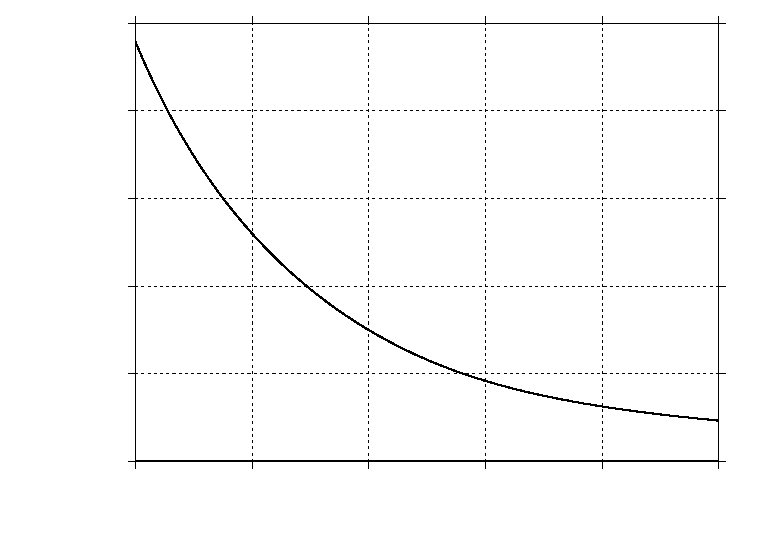
\includegraphics{Figures/TCrB/TCrB}}%
    \gplfronttext
  \end{picture}%
\endgroup
  
\caption{The critical temperatur $T_C$ is plotted as a function of the Bose gas parameter $(n_Ba_B^3)^{1/3}$. We observe a simple monotonic decrease with increasing gas parameter. Other parameters: $(n_Ba_{BF}^3)^{1/3} = 0.1, \frac{m_B}{m_F} = 7/40, \frac{n_F}{n_B^{1/3}} = 0.215$. }  
\label{fig.TCrB}  
\end{center}    
\end{figure}

In figure \ref{fig.TCrBF} we see the dependency of $T_C$ on the Bose-\textit{Fermi} gas parameter $(n_Ba_{BF}^3)^{1/3}$. This dependency is less trivial. For nonzero values of $T_C$ we see an expected rapid increase of $T_C$ with $(n_Ba_{BF}^3)^{1/3}$. This stems from the fact, that a higher value of the Bose-Fermi gas parameter gives a higher interaction strength between the fermions. The more puzzling part is the fact, that the critical temperature suddenly drops to zero at a cricitical value $(n_Ba_{BF}^3)_c^{1/3} \approx 0.059$. Hence, there is a critical value, that the interaction strength must be larger than, for any superconducting phase to appear. This is in stark contrast to the original s-wave BCS-theory, which has as one of its key features, that any nonzero attractive interaction between the fermions leads to a superconducting phase. 

\begin{figure} 
\begin{center}  
% GNUPLOT: LaTeX picture with Postscript
\begingroup
  \makeatletter
  \providecommand\color[2][]{%
    \GenericError{(gnuplot) \space\space\space\@spaces}{%
      Package color not loaded in conjunction with
      terminal option `colourtext'%
    }{See the gnuplot documentation for explanation.%
    }{Either use 'blacktext' in gnuplot or load the package
      color.sty in LaTeX.}%
    \renewcommand\color[2][]{}%
  }%
  \providecommand\includegraphics[2][]{%
    \GenericError{(gnuplot) \space\space\space\@spaces}{%
      Package graphicx or graphics not loaded%
    }{See the gnuplot documentation for explanation.%
    }{The gnuplot epslatex terminal needs graphicx.sty or graphics.sty.}%
    \renewcommand\includegraphics[2][]{}%
  }%
  \providecommand\rotatebox[2]{#2}%
  \@ifundefined{ifGPcolor}{%
    \newif\ifGPcolor
    \GPcolorfalse
  }{}%
  \@ifundefined{ifGPblacktext}{%
    \newif\ifGPblacktext
    \GPblacktexttrue
  }{}%
  % define a \g@addto@macro without @ in the name:
  \let\gplgaddtomacro\g@addto@macro
  % define empty templates for all commands taking text:
  \gdef\gplbacktext{}%
  \gdef\gplfronttext{}%
  \makeatother
  \ifGPblacktext
    % no textcolor at all
    \def\colorrgb#1{}%
    \def\colorgray#1{}%
  \else
    % gray or color?
    \ifGPcolor
      \def\colorrgb#1{\color[rgb]{#1}}%
      \def\colorgray#1{\color[gray]{#1}}%
      \expandafter\def\csname LTw\endcsname{\color{white}}%
      \expandafter\def\csname LTb\endcsname{\color{black}}%
      \expandafter\def\csname LTa\endcsname{\color{black}}%
      \expandafter\def\csname LT0\endcsname{\color[rgb]{1,0,0}}%
      \expandafter\def\csname LT1\endcsname{\color[rgb]{0,1,0}}%
      \expandafter\def\csname LT2\endcsname{\color[rgb]{0,0,1}}%
      \expandafter\def\csname LT3\endcsname{\color[rgb]{1,0,1}}%
      \expandafter\def\csname LT4\endcsname{\color[rgb]{0,1,1}}%
      \expandafter\def\csname LT5\endcsname{\color[rgb]{1,1,0}}%
      \expandafter\def\csname LT6\endcsname{\color[rgb]{0,0,0}}%
      \expandafter\def\csname LT7\endcsname{\color[rgb]{1,0.3,0}}%
      \expandafter\def\csname LT8\endcsname{\color[rgb]{0.5,0.5,0.5}}%
    \else
      % gray
      \def\colorrgb#1{\color{black}}%
      \def\colorgray#1{\color[gray]{#1}}%
      \expandafter\def\csname LTw\endcsname{\color{white}}%
      \expandafter\def\csname LTb\endcsname{\color{black}}%
      \expandafter\def\csname LTa\endcsname{\color{black}}%
      \expandafter\def\csname LT0\endcsname{\color{black}}%
      \expandafter\def\csname LT1\endcsname{\color{black}}%
      \expandafter\def\csname LT2\endcsname{\color{black}}%
      \expandafter\def\csname LT3\endcsname{\color{black}}%
      \expandafter\def\csname LT4\endcsname{\color{black}}%
      \expandafter\def\csname LT5\endcsname{\color{black}}%
      \expandafter\def\csname LT6\endcsname{\color{black}}%
      \expandafter\def\csname LT7\endcsname{\color{black}}%
      \expandafter\def\csname LT8\endcsname{\color{black}}%
    \fi
  \fi
    \setlength{\unitlength}{0.0500bp}%
    \ifx\gptboxheight\undefined%
      \newlength{\gptboxheight}%
      \newlength{\gptboxwidth}%
      \newsavebox{\gptboxtext}%
    \fi%
    \setlength{\fboxrule}{0.5pt}%
    \setlength{\fboxsep}{1pt}%
\begin{picture}(7200.00,5040.00)%
    \gplgaddtomacro\gplbacktext{%
      \csname LTb\endcsname%
      \put(946,767){\makebox(0,0)[r]{\strut{}$0$}}%
      \csname LTb\endcsname%
      \put(946,1415){\makebox(0,0)[r]{\strut{}$0.02$}}%
      \csname LTb\endcsname%
      \put(946,2062){\makebox(0,0)[r]{\strut{}$0.04$}}%
      \csname LTb\endcsname%
      \put(946,2710){\makebox(0,0)[r]{\strut{}$0.06$}}%
      \csname LTb\endcsname%
      \put(946,3357){\makebox(0,0)[r]{\strut{}$0.08$}}%
      \csname LTb\endcsname%
      \put(946,4005){\makebox(0,0)[r]{\strut{}$0.1$}}%
      \csname LTb\endcsname%
      \put(946,4652){\makebox(0,0)[r]{\strut{}$0.12$}}%
      \csname LTb\endcsname%
      \put(1141,484){\makebox(0,0){\strut{}$0$}}%
      \csname LTb\endcsname%
      \put(2261,484){\makebox(0,0){\strut{}$0.02$}}%
      \csname LTb\endcsname%
      \put(3381,484){\makebox(0,0){\strut{}$0.04$}}%
      \csname LTb\endcsname%
      \put(4500,484){\makebox(0,0){\strut{}$0.06$}}%
      \csname LTb\endcsname%
      \put(5620,484){\makebox(0,0){\strut{}$0.08$}}%
      \csname LTb\endcsname%
      \put(6740,484){\makebox(0,0){\strut{}$0.1$}}%
    }%
    \gplgaddtomacro\gplfronttext{%
      \csname LTb\endcsname%
      \put(176,2871){\rotatebox{-270}{\makebox(0,0){\strut{}$T_C/T_F$}}}%
      \put(3940,154){\makebox(0,0){\strut{}$(n_Ba_{BF}^3)^{1/3}$}}%
    }%
    \gplbacktext
    \put(0,0){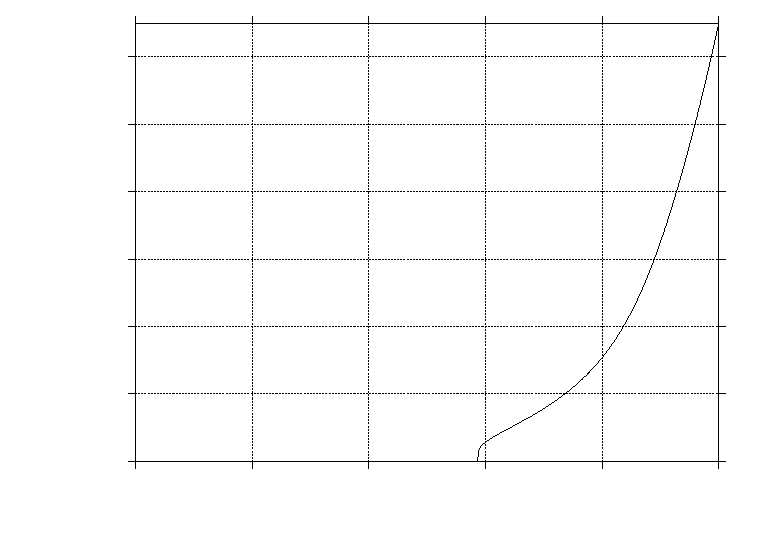
\includegraphics{Figures/TCrBF/TCrBF}}%
    \gplfronttext
  \end{picture}%
\endgroup
  
\caption{The critical temperatur $T_C$ is plotted as a function of the Bose-Fermi gas parameter $(n_Ba_{BF}^3)^{1/3}$. We see that, there is a cricital value of the gas parameter. Under this parameter the critical temperature vanishes. Other parameters: $(n_Ba_{B}^3)^{1/3} = 0.01, \frac{m_B}{m_F} = 7/40, \frac{n_F}{n_B^{1/3}} = 0.215$. }  
\label{fig.TCrBF}  
\end{center}    
\end{figure}



